\section{Versuchsaufbau und Durchführung}
\subsection{Aufgabe 1: Diagramme der Komponenten}
\section*{Beschreibung des Messsystems}
Das EKG-Messsystem basiert auf einem SparkFun RedBoard zur Datenerfassung und -verarbeitung. Die Herzaktivität wird über Elektroden aufgenommen, durch ein Sensormodul aufbereitet und anschließend über eine serielle Schnittstelle an einen PC zur Visualisierung übertragen. Die nachfolgenden Tabellen beschreiben die wesentlichen Komponenten sowie die verwendeten Signalpfade und Kommunikationsbussysteme, welche die Grundlage für die zu erstellenden Diagramme bilden.

\begin{figure}[H]
    \centering
    \includegraphics[width=1\textwidth]{figures/Messsystem.jpg}
    \caption{Blockschaltbild des EKG-Messsystems mit Signalfluss von links nach rechts.}
    \label{fig:blockschaltbild}
\end{figure}

\begin{figure}[H]
    \centering
    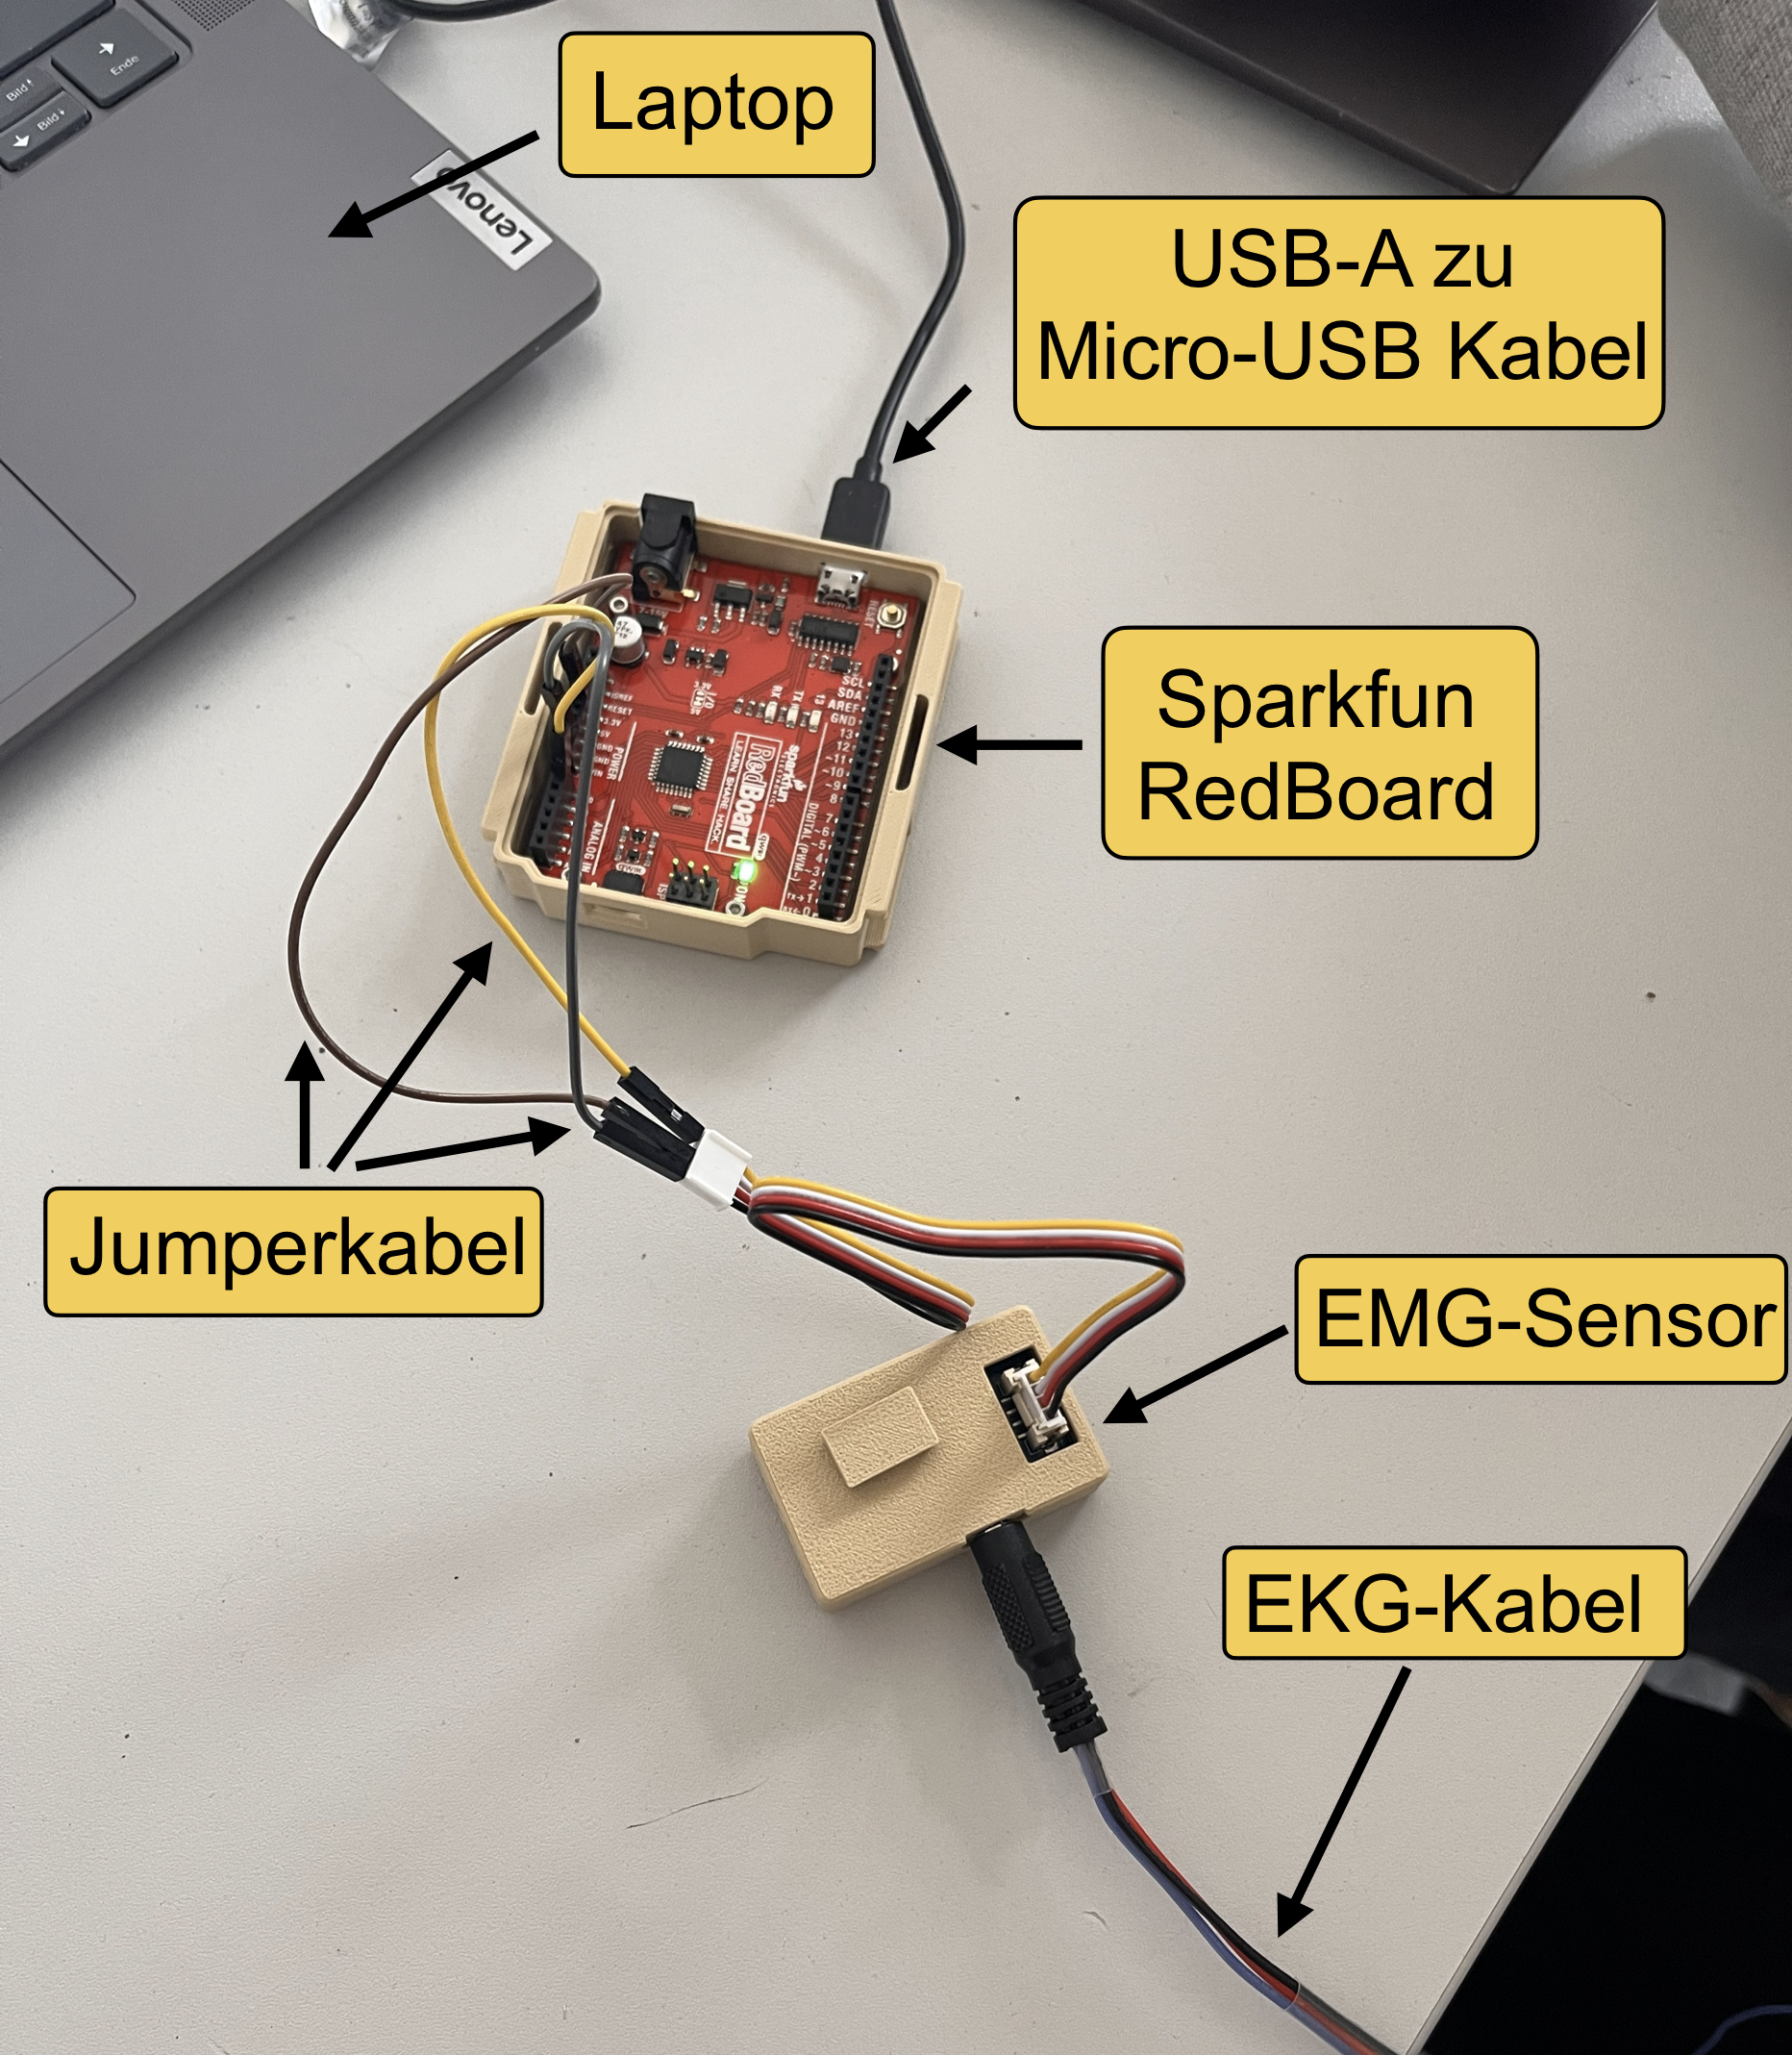
\includegraphics[width=0.4\textwidth]{figures/versuchsaufbau.png}
    \caption{Verbindung des EMG/EKG Sensors mit dem Sparkfun RedBoard Mikrocontroller}
    \label{fig:versuchsaufbau}
\end{figure}

\subsection*{Tabelle 1: Komponentenbeschreibungen}

\begin{table}[H]
    \centering
    \begin{tabular}{p{3.5cm} p{10cm}}
        \toprule
        Komponente & Beschreibung und Funktion \\
        \midrule
        EKG-Elektroden (Ag/AgCl) & Leitfähige Pads, die auf der Haut angebracht werden, um die biopotentiellen Spannungsdifferenzen des Herzens aufzunehmen und an das Sensorkabel weiterzuleiten. \\
        \midrule
        Sensormodul (AD8232) & Ein integrierter Signalaufbereitungsblock für EKG-Anwendungen. Er filtert Bewegungsartefakte und verstärkt das Millivolt-Signal auf einen für den Mikrocontroller lesbaren Pegel (0--3.3V oder 0--5V Output). \\
        \midrule
        SparkFun RedBoard (MCU) & Basiert auf dem ATmega328P Mikrocontroller (16 MHz). Er fungiert als ADC-Einheit, die das analoge Sensorsignal abtastet und digital verarbeitet. \\
        \midrule
        FTDI-Chip (Onboard) & Der FT231X Chip auf dem RedBoard wandelt die seriellen TTL-Signale des Mikrocontrollers in das USB-Protokoll um, damit der Computer diese lesen kann. \\
        \midrule
        Mini-USB Kabel & Physische Schnittstelle zur Übertragung der Daten vom FTDI-Chip zum PC sowie zur 5V-Stromversorgung des gesamten Boards. \\
        \midrule
        PC / Visualisierungssoftware & Empfängt den Datenstrom über den virtuellen COM-Port. Software (z.\,B. Serial Plotter oder Processing) stellt die Amplitudenwerte grafisch über der Zeit dar. \\
        \bottomrule
    \end{tabular}
    \label{tab:komponenten}
    \caption{Komponenten des EKG-Messsystems (Spezifikationen für SparkFun RedBoard).}
\end{table}

\subsection*{Tabelle 2: Signalpfade und Bussysteme}

\begin{table}[H]
    \centering
    \begin{tabular}{p{4cm} p{3cm} p{2.8cm} p{4cm}}
        \toprule
        Pfad / Verbindung &Bustyp / Signal & \textbf{Geschwindigkeit} & Technische Details \\
        \midrule
        Sensor $\rightarrow$ RedBoard Pin A0 & Analoges Spannungssignal & Kontinuierlich (Analog) & Übertragung der verstärkten Herzstromkurve als Spannungswert. \\
        \midrule
        Interne Verarbeitung (ATmega328P) & 10-Bit ADC Bus (Intern) & Abhängig vom Code (oft ca. 100-500 Hz Sampling) & Der interne ADC wandelt die Spannung in diskrete Integer-Werte von 0 bis 1023 um. \\
        \midrule
        ATmega328P $\rightarrow$ FTDI Chip & UART (TTL Seriell) & 500.000 Baud & Asynchrone serielle Übertragung über die RX/TX-Leitungen auf dem Board. \\
        \midrule
        RedBoard (USB) $\rightarrow$ PC & USB 2.0 (Virtual COM) & 12 Mbit/s (USB Full Speed) & Der FT231X Chip puffert die schnellen seriellen Daten und übergibt sie per USB an die Software. \\
        \bottomrule
    \end{tabular}
    \label{tab:signalpfade}
    \caption{Analyse der Signalpfade und Bus-Spezifikationen.}
\end{table}

\subsection{Aufgabe 2: Daten im Seriellen Plotter}
\subsection{Aufgabe 3: Experiment in Ruhe}
\subsection{Aufgabe 4: Beschreibung und Erklärung des Ruhe-EKG Codes}
\subsection{Aufgabe 5: Fünf-Sekunden-Plot der Ruhe-EKGs}
\subsection{Aufgabe 6: Errechnete Daten der Ruhe-EKGs}
\subsection{Aufgabe 7: Einordnung der Daten im Kontext derer der Mitstudierenden}
\subsection{Aufgabe 8: Plott der Herzfrequenz während des Belastungs-EKGs}
\subsection{Aufgabe 9: Ruhephase vor Belastungs-EKG}
\subsection{Aufgabe 10: Erholungsphase nach Belastungs-EKG}
\subsection{Aufgabe 11: Berechnen des metabolischen Energieverbrauchs}
\subsection{Aufgabe 12: Einordnung des Energieverbrauchs und entsprechender Code}